\section{ISAC相关的产业活动和研究成果}

\subsection{增强定位和跟踪}

从1G到未来的6G，定位一直是现有蜂窝网络标准化、部署和应用的关键特性。由于带宽​​和天线的限制分别导致距离和角度分辨率较低，目前大多数蜂窝网络（例如4G和5G）仅能提供米级精度的测量数据，以辅助全球导航卫星系统。根据5G新空口（NR）Release 17的关键参数指标，工业物联网应用中所需的最高定位精度为水平/垂直方向0.2米/1米，这无法满足未来应用的需求。尤其是在室内环境中，用户定位的精度要求高于室外环境，例如室内人体活动识别（~1厘米）、自主机器人和制造（~5毫米）。另一方面，目前的无线定位技术大多采用基于设备的方式，即将无线设备（例如智能手机）连接到待定位对象，通过与其他已部署的无线设备（例如Wi-Fi接入点或基站）的信号交互和几何关系来计算其位置。然而，这种基于设备的方法限制了定位对象的选择，并且无法推广到各种不同的场景。

得益于额外的多普勒处理和对多径分量有用信息的利用，支持ISAC的蜂窝网络能够实现比现有定位技术更高的定位精度。此外，具备感知功能的蜂窝网络不仅限于使用智能手机精确定位特定物体，还能应用于更广泛的场景，例如从周围环境中提取光谱和几何信息。

\subsection{区域成像}

射频成像技术能够生成高分辨率、全天候且不受天气影响的图像，可应用于环境监测、气候变化研究和安全应用等众多领域。值得注意的是，与基于摄像头的成像相比，射频成像的侵入性更小，能够聚焦于目标信息，而不会泄露周围环境中的敏感信息。由于上一代蜂窝系统带宽有限，其距离分辨率约为米级，无法支持高分辨率服务。得益于毫米波和MIMO技术的部署，未来的基站有望通过协同感知和成像特定区域，实现更高的距离和角度分辨率。在这种情况下，无线接入网将充当分布式MIMO雷达，详见第六节。因此，未来的蜂窝网络和用户设备能够“看到”周围环境，这将进一步支持数字孪生、虚拟现实等高层应用。此外，由于采用了更高的频率，成像分辨率显著提高，未来的蜂窝网络还将支持频谱图相关和空间/位置感知服务。最后，具备成像能力的蜂窝基站和用户设备可以为传统电信运营商带来额外的商业价值，例如为民用用户提供一种新的计费服务。

\subsection{车联网（V2X）}

自动驾驶汽车有望从根本上改变交通运输行业，提高高速公路通行能力和交通流量，降低油耗和污染，并有望减少交通事故。为了实现这一目标，车辆配备了通信收发器和各种传感器，旨在同时提取环境信息并与路侧单元、其他车辆甚至行人交换信息。传感和通信的结合已被证明是一条可行的途径，它减少了天线数量，缩小了系统尺寸，并降低了重量和功耗；这种结合缓解了电磁兼容性和频谱拥塞问题。例如，ISAC辅助的V2X通信可以提供环境信息，以支持快速车辆编队行驶、安全无缝的接入以及同步定位与地图构建。网络可以使传感服务扩展过往车辆的感知范围，使其超出自身的视距和视野。我们将简要讨论两个典型的应用案例。

\paragraph{a) 车辆编队行驶：}~\\

自动驾驶车辆以紧密间距的计算机控制车队形式存在，将提高高速公路通行能力并提升乘客舒适度。目前的车辆编队方案大多基于传统的领队-跟随者框架下的协同自适应巡航控制，这需要多跳车对车（V2V）通信来传输每辆车的状态信息。然而，多跳通信的高延迟会导致编队车辆的态势信息不同步，尤其是在车队很长且动态性很高的情况下。

\begin{figure}[htbp]
	\centering
	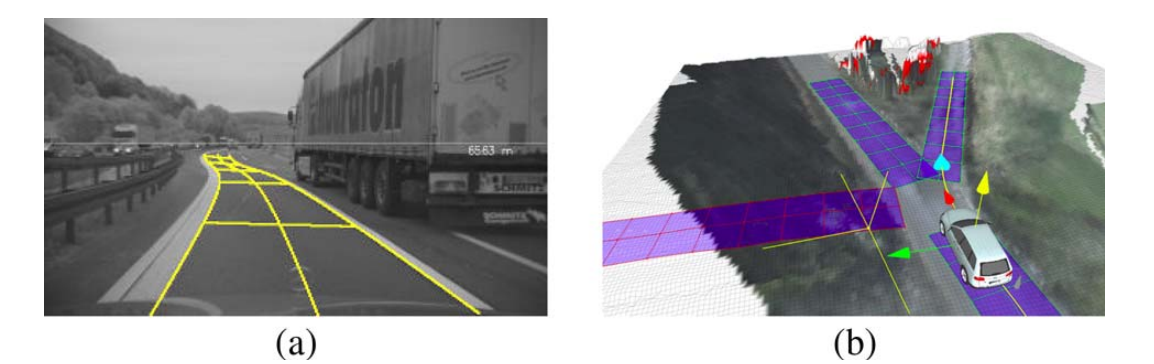
\includegraphics[width=0.9\linewidth]{img/5-1.png}
	\caption{(a) 在已标记的高速公路上进行车道跟踪(b)在实况路面环境中跟踪交叉路口}
	\label{fig:5-1}
\end{figure}

在这种情况下，无法感知态势变化的编队车辆会增加控制风险。路侧单元（RSU）作为车辆基础设施，能够同时服务于多辆车，因此为组建和维护车队提供了一种更可靠的方法。更重要的是，RSU上配备的无线传感功能提供了一种快速且廉价地获取车辆状态的替代方法，这反过来又通过显著降低波束训练开销和延迟来促进车路通信 和编队行驶。

\paragraph{b) 同步定位与建图（SLAM）：}~\\

联合定位与地图构建（SLAM）无需高精度地图即可为车辆提供态势感知能力。基于从各种传感器提取的环境数据，车辆可以获取其当前位置以及与局部区域内物体的空间关系，并据此进行导航和路径规划。以往的SLAM研究大多依赖于摄像头或激光雷达传感器，忽略了信道传播特性可用于构建周围环境的二维或三维地图这一事实。

\begin{figure}[htbp]
	\centering
	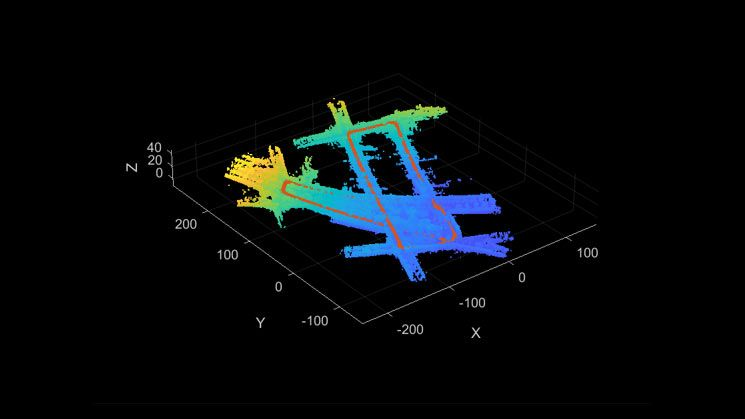
\includegraphics[width=0.7\linewidth]{img/5-2.jpg}
	\caption{常用于无人机和自动驾驶的三维点云 SLAM}
	\label{fig:5-1}
\end{figure}

从这个意义上讲，基于ISAC的无线电传感技术有望成为集成到现有SLAM解决方案中的关键组件，它能够赋予通信设备传感功能，同时只需对硬件/软件进行极少的修改。用于SLAM的ISAC接收信号处理流程面临诸多挑战，例如传感信号和通信信号的分离以及高质量点云的重建。

%a) 人类活动识别：
%活动识别对人类和计算机科学都至关重要，因为它能够记录人们的行为数据，使计算机系统能够监测、分析并辅助人们的日常生活。无线信号会受到静态和移动物体以及动态人体活动的影响。因此，无线信号的振幅和相位变化可用于检测或识别室内移动中的人体存在/接近/跌倒/睡眠/呼吸/日常活动，方法是提取距离、多普勒或微多普勒特征。此外，如果传感分辨率足够高，则可以通过识别驾驶员的眨眼频率来识别疲劳驾驶。通过将传感功能集成到当前的商用无线设备（例如 Wi-Fi 设备）中，这些技术能够检测和识别居民的活动，从而支持智能化和以人为本的生活环境。

%b) 空间感知计算：
%进一步挖掘海量物联网设备之间的几何关系，有望提升居民的福祉和居住舒适度，这正是空间感知计算技术的最终目标。高空间分辨率无线信号的普遍存在，为收集室内设备之间的所有空间关系提供了契机，这些设备可能密集且临时地部署在狭小的空间内。例如，一部具备厘米级传感精度的智能手机能够以±3°的角度分辨率精确定位任何电子设备。因此，只需将智能手机对准特定设备，即可实现二者之间的自动连接和控制。

此外，了解设备在空间和时间上的位置有助于更深入地了解邻近设备、网络和环境。通过考虑移动设备与接入点之间的空间关系，而非仅考虑信噪比，可以加快初始接入或跨网络切换操作。此外，空间感知计算有望协调以分布式方式部署的家用产品，共同分析移动情况、理解移动模式，并最终支持增强现实和虚拟现实应用。